\documentclass[border=2pt]{standalone}
% Shared preamble for standalone figures in this directory.
% Compile with XeLaTeX from 讲义/figs, or via the figures target.
\usepackage{ctex}
\usepackage{amsmath}
\usepackage{amssymb}
\usepackage{bm}
\usepackage{mathtools}
\usepackage{tikz}
\renewcommand{\vec}[1]{\boldsymbol{#1}}
\newcommand{\cC}{\mathcal{C}}
\newcommand{\cD}{\mathcal{D}}
\newcommand{\R}{\mathbf{R}}
\usetikzlibrary{
    arrows.meta,
    calc,
    decorations.markings,
    angles,
    quotes,
    positioning,
    patterns,
    shapes.geometric
}

\begin{document}
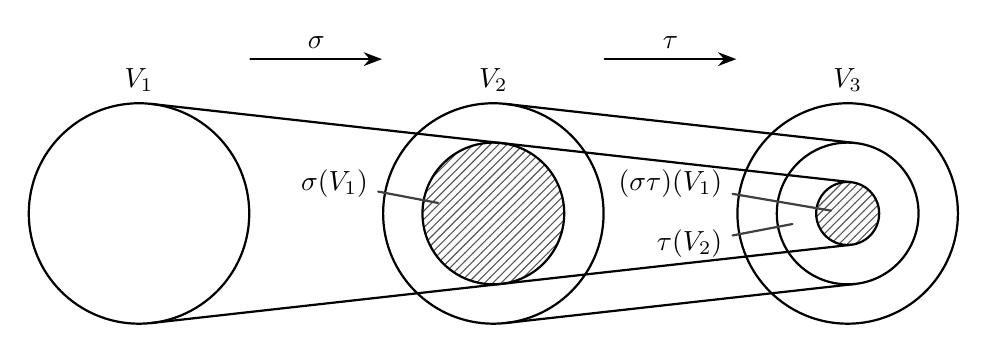
\begin{tikzpicture}[>=Stealth, thick, line cap=round,line join=round]
  \def\R{1.4}      % Radius R
  \def\a{0.5}      % Parameter a
  \def\d{4.5}      % Equal center-to-center spacing

  \tikzset{every pin edge/.style={darkgray, draw,thick,shorten <=-0.2cm}}

  % Derived radii
  \pgfmathsetmacro{\rmid}{\R-\a}     % radius of B2 and C2
  \pgfmathsetmacro{\rsmall}{\R-2*\a} % radius of C3
  \pgfmathsetmacro{\hh}{sqrt(\d*\d-\a*\a)}

  % Upper tangent
  \draw
    ({\a*\R/\d}, {\R*\hh/\d}) --
    ({2*\d+\a*\rsmall/\d}, {\rsmall*\hh/\d});

  % Lower tangent
  \draw
    ({\a*\R/\d}, {-\R*\hh/\d}) --
    ({2*\d+\a*\rsmall/\d}, {-\rsmall*\hh/\d});

  % A1
  \node[draw, circle, minimum size=2*\R cm, label=above:$V_1$] (A1) at (0, 0) {};

  % B1 and B2
  \node[draw, circle, minimum size=2*\R cm, label=above:$V_2$] (B1) at (\d, 0) {};
  \fill[pattern=north east lines,pattern color=black!65]
    (B1) circle[radius=\rmid];
  \node[draw, circle, minimum size=2*\rmid cm,
    pin={[pin distance=0.55cm]177:$\sigma(V_1)$}] (B2) at (B1) {};

  % C1, C2, C3
  \node[draw, circle, minimum size=2*\R cm, label=above:$V_3$] (C1) at (2*\d, 0) {};
  \node[draw, circle, minimum size=2*\rmid cm,
    pin={[pin distance=0.55cm]183:$\tau(V_2)$}] (C2) at (C1) {};
  \fill[pattern=north east lines,pattern color=black!65]
    (C1) circle[radius=\rsmall];
  \node[draw, circle, minimum size=2*\rsmall cm,
    pin={[pin distance=1.05cm]177:$(\sigma\tau)(V_1)$}] (C3) at (C1) {};

  \draw[->] ($(A1.east) + (0, 1.4*\R)$)
    -- ($(B1.west) + (0, 1.4*\R)$)
    node[midway, above] {$\sigma$};

  \draw[->] ($(B1.east) + (0, 1.4*\R)$)
    -- ($(C1.west) + (0, 1.4*\R)$)
    node[midway, above] {$\tau$};

  % Upper tangent
  \draw
    ({\d+\a*\R/\d}, {\R*\hh/\d}) --
    ({2*\d+\a*\rmid/\d}, {\rmid*\hh/\d});

  % Lower tangent
  \draw
    ({\d+\a*\R/\d}, {-\R*\hh/\d}) --
    ({2*\d+\a*\rmid/\d}, {-\rmid*\hh/\d});

\end{tikzpicture}

\end{document}
